\documentclass[a4paper,kulak]{kulakarticle}

\usepackage[utf8]{inputenc}
\usepackage[dutch]{babel}
\usepackage{pdfpages}
\usepackage{subfig}
\usepackage{float}

\usepackage{cite}

% style
%\usepackage[left=2.5cm,top=2cm,right=2.5cm,bottom=2cm,a4paper]{geometry}
\usepackage{color}

\date{\today}
\address{
	Bachelor in de fysica\\
	Bachelor in de informatica\\
	Bachelor in de wiskunde\\
	Ingenieurswetenschappen}
\title{BDA App}
\author{Marthe B\"{o}ting\\
	Robin Bruneel\\
	Toon Ingelaere}

\begin{document}
	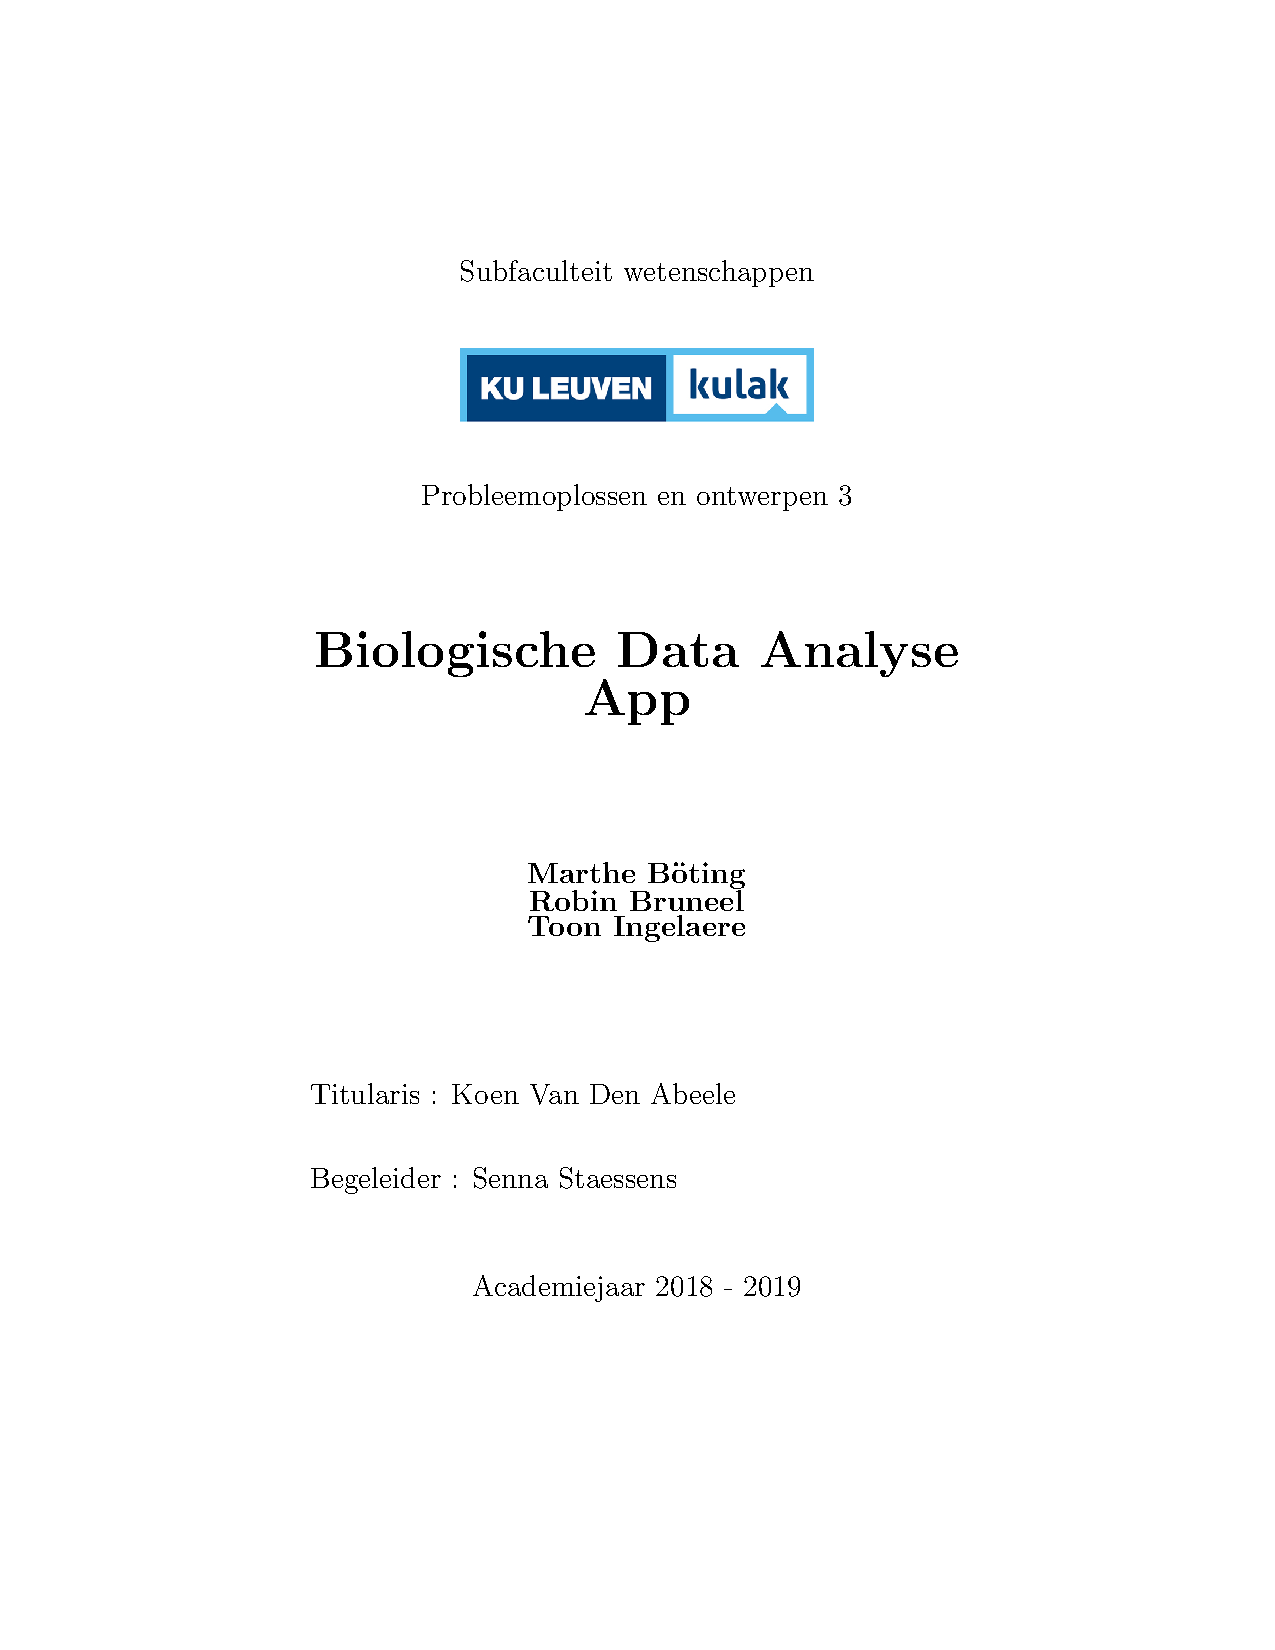
\includepdf{voorblad}
	
	\maketitle

\section*{Inleiding}

Inleidende tekst.
\pagebreak

%\tableofcontents

\section{Sectie-titel}

Tekst.

\section*{Besluit}

Afsluitende tekst

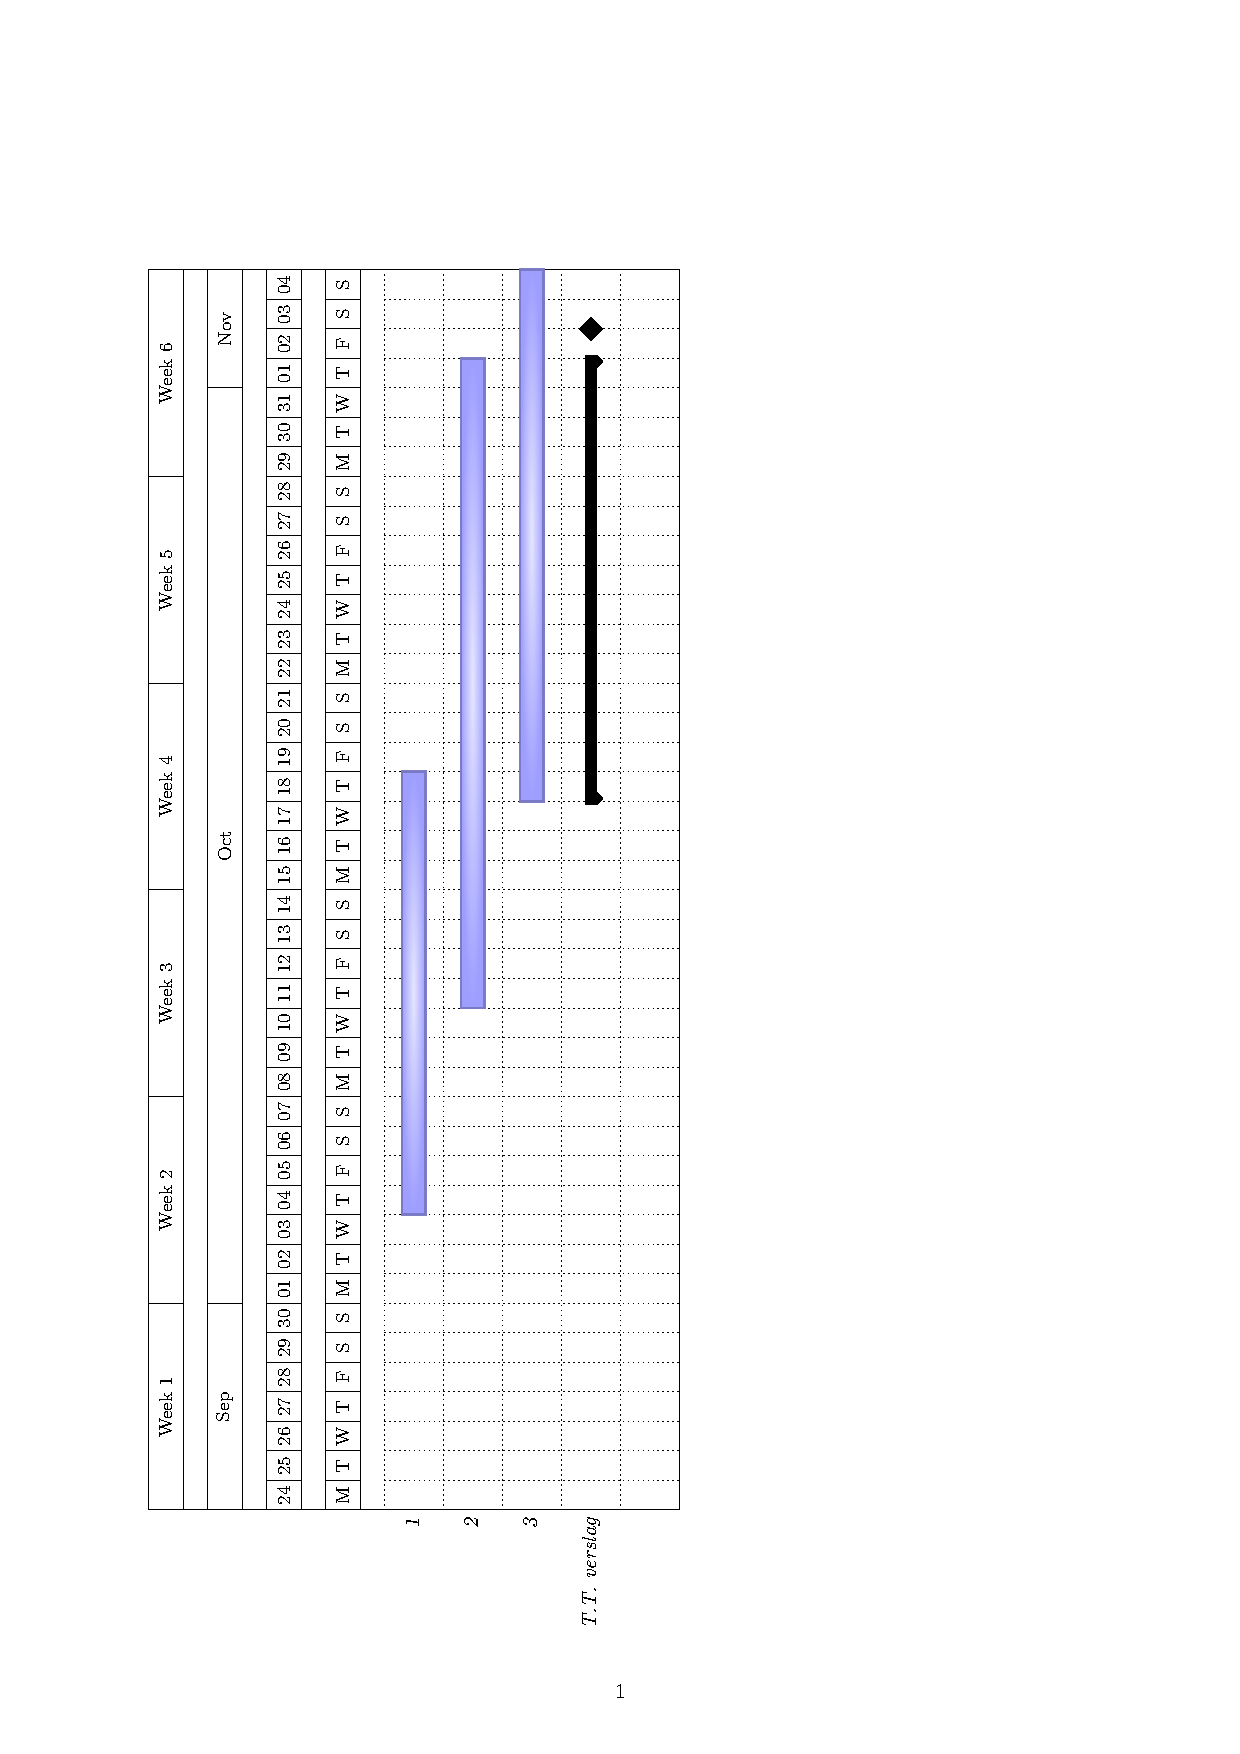
\includepdf[pages={1-3}]{ganttchart}

\end{document}
